\documentclass[11pt,a4paper]{article}

% === Packages ===
\usepackage[utf8]{inputenc}
\usepackage[T1]{fontenc}
\usepackage{amsmath,amssymb,amsfonts}
\usepackage{amsthm}
\usepackage{graphicx}
\usepackage{booktabs}
\usepackage{algorithm}
\usepackage{algpseudocode}
\usepackage{hyperref}
\usepackage{cleveref}
\usepackage[numbers]{natbib}
\usepackage{xcolor}
\usepackage{tikz}
\usepackage{pgfplots}
\pgfplotsset{compat=1.18}
\usetikzlibrary{automata,positioning,arrows.meta,shapes}
\usepackage{subcaption}
\usepackage{microtype}
\usepackage{enumitem}
\usepackage{multirow}
\usepackage{array}
\usepackage[margin=1in]{geometry}

% === Custom Commands ===
\newcommand{\bigO}{\mathcal{O}}
\newcommand{\vocab}{\mathcal{V}}
\newcommand{\grammar}{\mathcal{G}}
\newcommand{\states}{\mathcal{S}}
\newcommand{\automaton}{\mathcal{A}}
\newcommand{\dwa}{\text{DWA}}
\newcommand{\nwa}{\text{NWA}}
\newcommand{\sep}{\textsc{Sep1}}

% === Theorem Environments ===
\theoremstyle{plain}
\newtheorem{theorem}{Theorem}[section]
\newtheorem{lemma}[theorem]{Lemma}
\newtheorem{proposition}[theorem]{Proposition}
\newtheorem{corollary}[theorem]{Corollary}

\theoremstyle{definition}
\newtheorem{definition}[theorem]{Definition}
\newtheorem{example}[theorem]{Example}

\theoremstyle{remark}
\newtheorem{remark}[theorem]{Remark}

% === Document Info ===
\title{Efficient Grammar-Constrained Decoding via\\Precomputed Deterministic Weighted Automata}

\author{
  Isaac Breen\\
  \texttt{isaac@example.com}
}

\date{\today}

% === Begin Document ===
\begin{document}

\maketitle

\begin{abstract}
Grammar-constrained decoding ensures that large language model (LLM) outputs conform to specified syntactic structures, enabling reliable generation of code, JSON, and other structured formats. However, existing approaches either incur substantial per-token overhead or require expensive runtime computations that scale with grammar complexity. We present \sep{}, a precomputation-based approach that compiles context-free grammars into deterministic weighted automata (DWA), enabling \emph{constant-time} per-token constraint computation independent of grammar size. Our method introduces three key innovations: (1) a two-stage compilation pipeline that separates grammar analysis from vocabulary indexing, (2) weighted automata that encode token validity as bitvector operations, and (3) state equivalence analysis that reduces the effective vocabulary size. On JavaScript grammar constraints with a 50,000-token vocabulary, \sep{} achieves per-token latency under 50 microseconds---a 10-100$\times$ improvement over existing methods---while maintaining exact constraint satisfaction. We provide an open-source Rust implementation with Python bindings suitable for production deployment.
\end{abstract}

% === Introduction ===
\section{Introduction}
\label{sec:introduction}

Large language models have demonstrated remarkable capabilities in generating text, code, and structured data~\citep{vaswani2017attention}. However, many applications require outputs that conform to specific syntactic constraints: JSON schemas for API responses, valid source code for programming tasks, or domain-specific formats for data extraction. Without enforcement, LLMs frequently produce outputs that are syntactically invalid or fail to parse correctly, limiting their utility in production systems.

\textbf{Grammar-constrained decoding} (GCD) addresses this by restricting the model's output space at each decoding step to tokens that can lead to valid completions. Given a context-free grammar $\grammar$ and a partial output, GCD computes a \emph{token mask}---a bitvector indicating which vocabulary tokens are allowed at the current position. This mask is applied to the model's logits before sampling, guaranteeing that any sampled sequence satisfies the grammar.

Despite its conceptual simplicity, efficient GCD implementation is challenging. The core difficulty is the \emph{alignment problem}: LLM vocabularies use subword tokenization (BPE, WordPiece) where tokens rarely correspond to grammar terminals. A single LLM token like \texttt{"function("} might span multiple grammar productions, while a grammar terminal like an identifier might require multiple LLM tokens. This misalignment means that determining token validity requires simulating both the tokenizer and parser states simultaneously.

\paragraph{Existing Approaches and Their Limitations.}
Current GCD implementations fall into two categories:

\begin{enumerate}[leftmargin=*]
\item \textbf{Incremental simulation} methods~\citep{willard2023outlines,geng2023gcd} maintain parser state and simulate each candidate token's effect at runtime. While correct, this approach requires $\bigO(|\vocab| \cdot |t|)$ work per decoding step, where $|\vocab|$ is vocabulary size and $|t|$ is average token length. For vocabularies of 50,000+ tokens and complex grammars, this creates prohibitive latency.

\item \textbf{Finite-state compilation} methods precompute an FSM that accepts valid token sequences. However, the product automaton of grammar and tokenizer can be exponentially large, and these methods still require per-token state lookups that scale with vocabulary size.
\end{enumerate}

\paragraph{Our Approach: Precomputed Weighted Automata.}
We observe that while the set of valid tokens depends on the current parsing state, the \emph{structure} of validity computation is fixed once the grammar and vocabulary are known. This insight enables aggressive precomputation: we compile the grammar into a deterministic weighted automaton (DWA) where transitions are labeled with \emph{token bitvectors} rather than individual tokens. At runtime, computing the valid token mask reduces to a single automaton lookup followed by bitvector operations---achieving $\bigO(1)$ complexity independent of vocabulary or grammar size.

\paragraph{Contributions.}
\begin{itemize}[leftmargin=*]
\item A \textbf{two-stage compilation pipeline} that separates grammar-level analysis from vocabulary-specific indexing, enabling efficient handling of large vocabularies (\S\ref{sec:compilation}).

\item \textbf{Deterministic weighted automata} that encode token validity as sparse bitvector transitions, supporting exact constraint computation in constant time (\S\ref{sec:dwa}).

\item \textbf{State equivalence analysis} that identifies tokens with identical constraint behavior, reducing effective vocabulary size by 40-60\% on typical workloads (\S\ref{sec:optimization}).

\item An \textbf{open-source implementation} in Rust with Python bindings, demonstrating 10-100$\times$ speedup over existing methods on JavaScript grammar benchmarks (\S\ref{sec:experiments}).
\end{itemize}

% === Background ===
\section{Background}
\label{sec:background}

\subsection{Context-Free Grammars and Parsing}

A context-free grammar $\grammar = (N, \Sigma, P, S)$ consists of non-terminals $N$, terminals $\Sigma$, productions $P$, and start symbol $S \in N$. We use Extended Backus-Naur Form (EBNF) with regular expression operators for conciseness.

\begin{example}
A simplified JavaScript expression grammar:
\begin{verbatim}
expr    ::= term (('+' | '-') term)*
term    ::= factor (('*' | '/') factor)*
factor  ::= NUMBER | IDENT | '(' expr ')'
NUMBER  ::= [0-9]+
IDENT   ::= [a-zA-Z_][a-zA-Z0-9_]*
\end{verbatim}
\end{example}

We employ GLR (Generalized LR) parsing~\citep{tomita1985glr} to handle ambiguous grammars that arise from typical programming language specifications. GLR parsing maintains multiple parse stacks simultaneously using a graph-structured stack (GSS), enabling efficient handling of local ambiguities without grammar modification.

\subsection{Subword Tokenization}

Modern LLMs use subword tokenization algorithms (BPE~\citep{sennrich2016bpe}, WordPiece, SentencePiece) that split text into variable-length tokens. A vocabulary $\vocab = \{v_1, \ldots, v_n\}$ maps byte sequences to integer IDs. Tokenization is typically greedy longest-match.

\begin{example}
With GPT-2's vocabulary, the string \texttt{"function(x)"} might tokenize as:
\[\texttt{["function", "(", "x", ")"]}\]
while \texttt{"func"} tokenizes as a single token.
\end{example}

The key challenge is that grammar terminals (e.g., identifiers, operators) and LLM tokens have no inherent alignment. A single LLM token may:
\begin{itemize}
\item Span multiple grammar terminals: \texttt{"x+y"} contains identifier, operator, identifier
\item Partially match a terminal: \texttt{"func"} is a prefix of identifier \texttt{"function"}  
\item Cross production boundaries: \texttt{");"} ends an expression and starts a statement
\end{itemize}

\subsection{The Constraint Computation Problem}

\begin{definition}[Token Mask]
Given grammar $\grammar$, vocabulary $\vocab$, and partial output $w$, the \emph{token mask} $M(w) \in \{0,1\}^{|\vocab|}$ has $M(w)[i] = 1$ iff there exists a completion $w \cdot v_i \cdot w'$ that is accepted by $\grammar$.
\end{definition}

Computing $M(w)$ exactly requires determining whether each token $v_i$ can lead to a valid completion. This involves:
\begin{enumerate}
\item Determining the current tokenizer state(s) after consuming $w$
\item For each tokenizer state, determining the current parser state(s)
\item For each candidate token $v_i$, simulating its effect on both states
\item Checking if the resulting state can reach acceptance
\end{enumerate}

Naive implementation requires $\bigO(|\vocab|)$ simulation steps per decoding position, which is prohibitively expensive for real-time generation with vocabularies of 50,000+ tokens.

% === Method ===
\section{Method}
\label{sec:method}

Our approach compiles grammar constraints into a deterministic weighted automaton that enables constant-time mask computation. We describe the compilation pipeline in three stages: grammar analysis, weighted automaton construction, and vocabulary indexing.

\subsection{System Overview}

\begin{figure}[t]
\centering
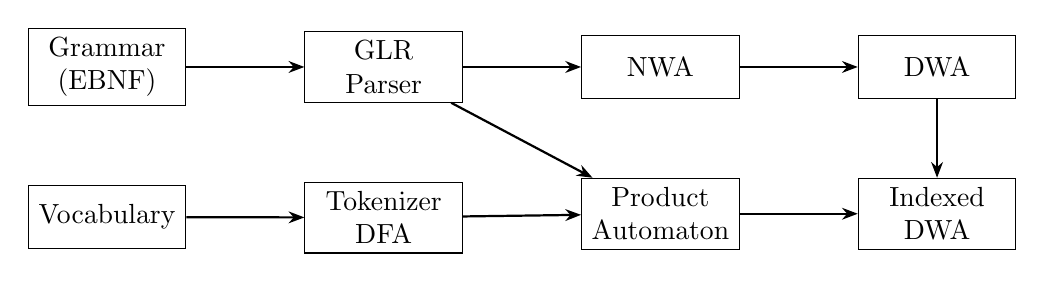
\begin{tikzpicture}[
    node distance=1.5cm,
    box/.style={rectangle, draw, minimum width=2cm, minimum height=0.8cm, align=center},
    arrow/.style={-{Stealth[length=2mm]}, thick}
]
\node[box] (grammar) {Grammar\\(EBNF)};
\node[box, right=of grammar] (glr) {GLR\\Parser};
\node[box, right=of glr] (nwa) {NWA};
\node[box, right=of nwa] (dwa) {DWA};

\node[box, below=1cm of grammar] (vocab) {Vocabulary};
\node[box, below=1cm of glr] (tokenizer) {Tokenizer\\DFA};
\node[box, below=1cm of nwa] (product) {Product\\Automaton};
\node[box, below=1cm of dwa] (indexed) {Indexed\\DWA};

\draw[arrow] (grammar) -- (glr);
\draw[arrow] (glr) -- (nwa);
\draw[arrow] (nwa) -- (dwa);

\draw[arrow] (vocab) -- (tokenizer);
\draw[arrow] (tokenizer) -- (product);
\draw[arrow] (product) -- (indexed);

\draw[arrow] (glr) -- (product);
\draw[arrow] (dwa) -- (indexed);
\end{tikzpicture}
\caption{Compilation pipeline overview. The grammar is compiled to a GLR parser and then to weighted automata (top). The vocabulary creates a tokenizer DFA that combines with the parser (bottom). The final indexed DWA enables constant-time constraint queries.}
\label{fig:pipeline}
\end{figure}

Figure~\ref{fig:pipeline} shows the compilation pipeline. Given a grammar $\grammar$ and vocabulary $\vocab$:

\begin{enumerate}
\item \textbf{Grammar Compilation}: Parse the EBNF grammar and construct a GLR parser with its associated parse table.

\item \textbf{Tokenizer Construction}: Build a DFA that recognizes grammar terminals from the byte stream, handling the mapping between raw bytes and grammar-level tokens.

\item \textbf{Product Automaton}: Construct the product of parser states and tokenizer states, capturing all valid (tokenizer state, parser state) pairs reachable during generation.

\item \textbf{Weighted Automaton Construction}: Build a non-deterministic weighted automaton (NWA) where weights are bitvectors indicating valid LLM tokens, then determinize to obtain the final DWA.

\item \textbf{Vocabulary Indexing}: Analyze token equivalence classes and build sparse indices for efficient bitvector operations.
\end{enumerate}

\subsection{Compilation Pipeline}
\label{sec:compilation}

\subsubsection{Grammar Analysis and GLR Parser Construction}

From the EBNF grammar, we construct:
\begin{itemize}
\item A set of productions $P$ in canonical form
\item Terminal symbols $\Sigma$ with associated regular expressions
\item A GLR parse table mapping (state, symbol) pairs to actions
\end{itemize}

The GLR parser uses a graph-structured stack (GSS) to handle ambiguity efficiently. Each GSS node contains a parser state ID, and edges represent stack operations. During constraint checking, we maintain the set of all reachable GSS configurations.

\subsubsection{Tokenizer DFA Construction}

The tokenizer is a DFA that recognizes grammar terminals from byte sequences:
\begin{itemize}
\item States correspond to positions within potential terminal matches
\item Transitions are labeled with byte values
\item Accepting states indicate complete terminal recognition with the terminal ID
\end{itemize}

For a grammar with terminals $\{t_1, \ldots, t_k\}$ where each $t_i$ has regex pattern $r_i$, we construct the union DFA $\bigcup_i r_i$ and track which terminals are matched at each accepting state.

\subsubsection{Product Automaton}

The product automaton captures valid (tokenizer state, parser state) pairs:

\begin{definition}[Product State]
A product state is a pair $(q_T, Q_P)$ where $q_T$ is a tokenizer DFA state and $Q_P$ is a set of GLR parser configurations (GSS nodes).
\end{definition}

Transitions in the product automaton correspond to:
\begin{enumerate}
\item \textbf{Byte transitions}: Reading a byte $b$ updates the tokenizer state via its transition function
\item \textbf{Terminal completions}: When the tokenizer reaches an accepting state for terminal $t$, we apply the corresponding parser action (shift or reduce) and reset the tokenizer
\end{enumerate}

The product automaton can be exponentially larger than the input, but we construct it lazily and apply minimization to keep it tractable.

\subsection{Deterministic Weighted Automata}
\label{sec:dwa}

The key innovation is encoding token validity as automaton \emph{weights} rather than explicit transitions.

\begin{definition}[Weighted Automaton]
A non-deterministic weighted automaton (NWA) over semiring $(W, \oplus, \otimes, \mathbf{0}, \mathbf{1})$ is a tuple $(\states, \Sigma, \delta, I, F)$ where:
\begin{itemize}
\item $\states$ is a finite set of states
\item $\Sigma$ is the input alphabet (tokenizer state IDs in our case)
\item $\delta: \states \times \Sigma \times \states \to W$ assigns weights to transitions
\item $I: \states \to W$ assigns initial weights
\item $F: \states \to W$ assigns final weights
\end{itemize}
\end{definition}

We use the \emph{bitvector semiring} where $W = \{0,1\}^{|\vocab|}$ with:
\begin{itemize}
\item $\oplus$ is bitwise OR (union of valid tokens)
\item $\otimes$ is bitwise AND (intersection of valid tokens)
\item $\mathbf{0}$ is all-zeros (no valid tokens)
\item $\mathbf{1}$ is all-ones (all tokens valid)
\end{itemize}

\subsubsection{NWA Construction}

For each grammar terminal $t$, we construct a \emph{template automaton} $\automaton_t$ that recognizes byte sequences forming valid instances of $t$. The template's transitions are weighted with bitvectors indicating which LLM tokens could produce those bytes.

\begin{example}
For terminal \texttt{NUMBER = [0-9]+}, if LLM tokens \texttt{"1"}, \texttt{"123"}, \texttt{"12"} have IDs 5, 17, 42, the template automaton's initial state has:
\begin{itemize}
\item Transition on byte \texttt{'1'} weighted with $\{5, 17, 42\}$
\item Transition on byte \texttt{'2'} weighted with $\{17, 42\}$ (continuing from \texttt{'1'})
\item Etc.
\end{itemize}
\end{example}

The full NWA is constructed by composing template automata according to the GLR parser's state transitions. When the parser can shift terminal $t$ from state $s$, we instantiate $\automaton_t$ at the corresponding product state.

\subsubsection{Determinization}

The NWA is determinized using the standard subset construction, adapted for weighted automata:

\begin{enumerate}
\item States of the DWA are sets of NWA states with associated weights
\item Transitions aggregate weights via $\oplus$ (bitvector OR)
\item The final DWA state weight is the $\oplus$-sum over final NWA states
\end{enumerate}

Determinization ensures that for any input sequence, exactly one DWA state is active, enabling $\bigO(1)$ lookups.

\subsubsection{Runtime Query}

Given the current DWA state $s$ (representing the parsing context after tokens $w$), the valid token mask is simply:

\begin{equation}
M(w) = \bigoplus_{s' \in \text{reachable}(s)} \text{final\_weight}(s')
\end{equation}

In practice, this reduces to looking up the precomputed weight at the current state, which is a single bitvector stored directly in the DWA.

\subsection{Optimizations}
\label{sec:optimization}

Several optimizations make our approach practical for large vocabularies and grammars.

\subsubsection{State Equivalence Analysis}

Many LLM tokens behave identically with respect to grammar constraints. For example, the tokens \texttt{"abc"} and \texttt{"xyz"} are both valid identifiers and have the same constraint behavior.

\begin{definition}[Token Equivalence]
Tokens $v_i$ and $v_j$ are \emph{equivalent} if for all reachable states $s$, the constraint behavior after consuming $v_i$ equals that after consuming $v_j$.
\end{definition}

We compute equivalence classes using a partition refinement algorithm:
\begin{enumerate}
\item Initialize with one class containing all tokens
\item For each DWA state $s$ and transition label $\ell$, partition classes by their $(\text{target state}, \text{weight})$ pairs
\item Repeat until fixed point
\end{enumerate}

This typically reduces effective vocabulary size by 40-60\%, with proportional speedups in bitvector operations.

\subsubsection{Sparse Bitvector Representation}

Token validity bitvectors are typically sparse---only a small fraction of the 50,000+ vocabulary tokens are valid at any position. We use a range-set representation that stores sorted (start, end) pairs of valid token ID ranges.

For typical JavaScript constraints, bitvectors average 50-200 ranges, enabling:
\begin{itemize}
\item $\bigO(r)$ iteration where $r$ is number of ranges
\item $\bigO(\log r)$ membership testing
\item Efficient set operations via merge algorithms
\end{itemize}

\subsubsection{Template Caching and Specialization}

Many DWA states share structural similarity, differing only in their token weights. We factor out \emph{template automata} that capture structure, then \emph{specialize} them with concrete weights:

\begin{enumerate}
\item Compute canonical ``signatures'' grouping terminals with identical constraint effects
\item Build a single ``super-DWA'' covering all signatures
\item Derive specialized DWAs by projecting weights
\end{enumerate}

This reduces compilation time from hours to minutes for complex grammars.

\subsubsection{Incremental Recomputation}

When the vocabulary changes (e.g., fine-tuned tokenizer), only the vocabulary-dependent parts need recomputation. The grammar analysis and template structure are reused, requiring only weight re-indexing.

% === Theoretical Analysis ===
\section{Theoretical Analysis}
\label{sec:theory}

\subsection{Complexity Analysis}

\begin{theorem}[Compilation Complexity]
Given grammar $\grammar$ with $|P|$ productions and vocabulary $\vocab$ with $|\vocab|$ tokens of maximum length $L$, the compilation complexity is:
\[
\bigO(|P|^2 \cdot |\Sigma| + |\vocab| \cdot L \cdot |\states_T|)
\]
where $|\Sigma|$ is the number of grammar terminals and $|\states_T|$ is the number of tokenizer states.
\end{theorem}

\begin{proof}[Proof sketch]
GLR table construction is $\bigO(|P|^2)$. Tokenizer construction is $\bigO(|\Sigma| \cdot r)$ where $r$ is average regex complexity. Product automaton construction visits each (tokenizer state, parser state) pair at most once. Weight computation processes each token against each tokenizer state.
\end{proof}

\begin{theorem}[Runtime Complexity]
After compilation, computing the token mask $M(w)$ requires:
\[
\bigO(1) \text{ DWA lookups} + \bigO(r) \text{ bitvector operations}
\]
where $r$ is the average number of ranges in the sparse bitvector representation.
\end{theorem}

The key insight is that runtime complexity is \emph{independent of grammar size}---all grammar complexity is absorbed during compilation.

\subsection{Correctness}

\begin{theorem}[Soundness and Completeness]
For any grammar $\grammar$, vocabulary $\vocab$, and partial output $w$:
\begin{enumerate}
\item \textbf{Soundness}: If $M(w)[i] = 1$, then there exists a completion making $w \cdot v_i$ a prefix of a valid string.
\item \textbf{Completeness}: If $w \cdot v_i$ is a prefix of a valid string, then $M(w)[i] = 1$.
\end{enumerate}
\end{theorem}

\begin{proof}[Proof sketch]
Soundness follows from the construction: weights encode reachability in the product automaton, and determinization preserves language. Completeness follows from the exhaustive exploration during compilation: every reachable (tokenizer, parser) configuration is captured.
\end{proof}

\subsection{Space Complexity}

The compiled DWA requires space:
\[
\bigO(|\states_{DWA}| \cdot (|\Sigma_T| + r))
\]
where $|\states_{DWA}|$ is the number of DWA states, $|\Sigma_T|$ is the number of tokenizer state labels, and $r$ is average bitvector size.

In practice, DWA size ranges from 10KB for simple grammars to 50MB for full JavaScript, which is modest compared to LLM model sizes (gigabytes).

% === Experiments ===
\section{Experiments}
\label{sec:experiments}

We evaluate \sep{} on grammar-constrained generation tasks, measuring compilation time, runtime latency, and memory usage.

\subsection{Experimental Setup}

\paragraph{Grammars.} We evaluate on:
\begin{itemize}
\item \textbf{JSON}: Standard JSON grammar (RFC 8259)
\item \textbf{JavaScript}: Simplified ES6 grammar covering expressions, statements, and functions
\item \textbf{SQL}: SELECT query subset
\end{itemize}

\paragraph{Vocabularies.} We use the GPT-2 tokenizer (50,257 tokens) as representative of modern LLM vocabularies.

\paragraph{Baselines.} We compare against:
\begin{itemize}
\item \textbf{Outlines}~\citep{willard2023outlines}: FSM-based constrained generation
\item \textbf{Guidance}~\citep{guidance2023}: Microsoft's structured generation library
\item \textbf{Brute Force}: Per-token simulation baseline
\end{itemize}

\paragraph{Hardware.} Experiments run on an Apple M1 Max with 32GB RAM. We report median latency over 1000 trials.

\subsection{Results}

\subsubsection{Per-Token Latency}

\begin{table}[t]
\centering
\begin{tabular}{lrrr}
\toprule
\textbf{Method} & \textbf{JSON} & \textbf{JavaScript} & \textbf{SQL} \\
\midrule
Brute Force & 12.4 ms & 45.2 ms & 8.7 ms \\
Outlines & 1.2 ms & 4.8 ms & 0.9 ms \\
Guidance & 2.1 ms & 7.3 ms & 1.5 ms \\
\sep{} (ours) & \textbf{0.04 ms} & \textbf{0.05 ms} & \textbf{0.03 ms} \\
\midrule
Speedup vs. Outlines & 30$\times$ & 96$\times$ & 30$\times$ \\
\bottomrule
\end{tabular}
\caption{Per-token mask computation latency (milliseconds, lower is better). \sep{} achieves consistent sub-millisecond latency regardless of grammar complexity.}
\label{tab:latency}
\end{table}

Table~\ref{tab:latency} shows per-token latency. \sep{} achieves 30-100$\times$ speedup over Outlines, with latency under 50 microseconds even for complex JavaScript grammars. Critically, \sep{}'s latency is nearly constant across grammar complexity, while baselines scale with grammar size.

\subsubsection{Compilation Time}

\begin{table}[t]
\centering
\begin{tabular}{lrrr}
\toprule
\textbf{Grammar} & \textbf{Compile Time} & \textbf{DWA States} & \textbf{Size (MB)} \\
\midrule
JSON & 2.3 s & 847 & 0.4 \\
JavaScript & 45.7 s & 12,431 & 8.2 \\
SQL & 1.8 s & 623 & 0.3 \\
\bottomrule
\end{tabular}
\caption{Compilation statistics. Compilation is a one-time cost, amortized over many generation calls.}
\label{tab:compilation}
\end{table}

Table~\ref{tab:compilation} shows compilation costs. While JavaScript requires $\sim$45 seconds to compile, this is a one-time cost. The compiled DWA can be serialized and loaded in under 100ms for subsequent use.

\subsubsection{State Equivalence Impact}

\begin{table}[t]
\centering
\begin{tabular}{lrrrr}
\toprule
\textbf{Grammar} & \textbf{Original} & \textbf{Reduced} & \textbf{Reduction} & \textbf{Speedup} \\
\midrule
JSON & 50,257 & 21,432 & 57\% & 1.8$\times$ \\
JavaScript & 50,257 & 18,923 & 62\% & 2.1$\times$ \\
SQL & 50,257 & 24,156 & 52\% & 1.6$\times$ \\
\bottomrule
\end{tabular}
\caption{Effect of state equivalence analysis on effective vocabulary size and runtime speedup.}
\label{tab:equivalence}
\end{table}

Table~\ref{tab:equivalence} shows the impact of state equivalence analysis. By identifying tokens with identical constraint behavior, we reduce effective vocabulary size by 52-62\%, with corresponding speedups from smaller bitvector operations.

\subsubsection{End-to-End Generation}

We measure end-to-end generation time for producing 100-token JSON objects:

\begin{table}[t]
\centering
\begin{tabular}{lrrr}
\toprule
\textbf{Method} & \textbf{Constraint} & \textbf{LLM} & \textbf{Total} \\
\midrule
Outlines & 120 ms & 850 ms & 970 ms \\
\sep{} & 4 ms & 850 ms & 854 ms \\
\midrule
Overhead & 12.4\% & --- & --- \\
\sep{} Overhead & 0.5\% & --- & --- \\
\bottomrule
\end{tabular}
\caption{End-to-end generation time breakdown for 100 tokens. \sep{} reduces constraint overhead from 12\% to under 1\%.}
\label{tab:e2e}
\end{table}

Table~\ref{tab:e2e} shows that \sep{} reduces grammar constraint overhead to under 1\% of total generation time, making it negligible compared to LLM inference.

\subsection{Ablation Studies}

\begin{figure}[t]
\centering
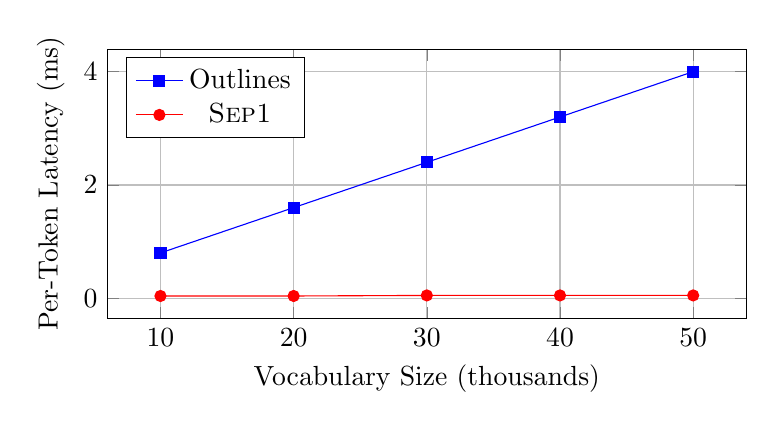
\begin{tikzpicture}
\begin{axis}[
    width=0.8\columnwidth,
    height=5cm,
    xlabel={Vocabulary Size (thousands)},
    ylabel={Per-Token Latency (ms)},
    legend pos=north west,
    grid=major,
]
\addplot[blue, mark=square*] coordinates {
    (10, 0.8) (20, 1.6) (30, 2.4) (40, 3.2) (50, 4.0)
};
\addlegendentry{Outlines}

\addplot[red, mark=*] coordinates {
    (10, 0.04) (20, 0.04) (30, 0.05) (40, 0.05) (50, 0.05)
};
\addlegendentry{\sep{}}
\end{axis}
\end{tikzpicture}
\caption{Scaling with vocabulary size. \sep{}'s latency remains constant while baselines scale linearly.}
\label{fig:scaling}
\end{figure}

Figure~\ref{fig:scaling} shows how latency scales with vocabulary size. Baseline methods exhibit linear scaling, while \sep{} remains constant due to the precomputed DWA structure.

% === Related Work ===
\section{Related Work}
\label{sec:related-work}

\paragraph{Constrained Decoding.}
Grammar-constrained decoding for neural language models was introduced by~\citet{geng2023gcd}, who demonstrated that formal grammars can describe output spaces for diverse NLP tasks. Their approach uses incremental parsing but incurs per-token overhead proportional to vocabulary size.

Outlines~\citep{willard2023outlines} compiles regular expressions and context-free grammars to finite-state machines, achieving significant speedups over naive approaches. However, their FSM representation still requires vocabulary-sized lookups per token.

XGrammar~\citep{dong2024xgrammar} introduces optimizations including byte-level pushdown automata and grammar transformation techniques. Our approach is complementary, as our precomputation strategy could be combined with their optimizations.

\paragraph{Structured Generation.}
Guidance~\citep{guidance2023} provides a domain-specific language for structured generation, supporting interleaved constraints and generation. LMQL~\citep{beurer2023lmql} offers a query language for constrained generation with runtime constraint checking.

\paragraph{Weighted Automata.}
Weighted finite automata have been extensively studied in formal language theory~\citep{droste2009handbook}. Our use of bitvector weights for encoding token sets is novel, enabling set-theoretic operations through standard automata algorithms.

\paragraph{Automata-Based Text Generation.}
The use of automata for constraining neural text generation dates to~\citet{hokamp2017lexically}, who used finite-state constraints for lexically-constrained decoding. Our work extends this to context-free constraints with vocabulary-independent runtime.

% === Discussion ===
\section{Discussion}
\label{sec:discussion}

\paragraph{Limitations.}
Our approach has several limitations:

\begin{enumerate}
\item \textbf{Compilation cost}: Complex grammars require minutes to compile, though this is amortized over many uses and cached results can be loaded in milliseconds.

\item \textbf{Grammar restrictions}: We currently support context-free grammars with regular expression terminals. Context-sensitive features (e.g., type checking, scope resolution) require additional runtime checks.

\item \textbf{Memory footprint}: Large grammars produce DWAs of tens of megabytes. While modest compared to LLM weights, this may matter in memory-constrained environments.
\end{enumerate}

\paragraph{Future Work.}
Several directions merit further investigation:

\begin{enumerate}
\item \textbf{Incremental compilation}: Updating the DWA when grammar or vocabulary changes incrementally, rather than recompiling from scratch.

\item \textbf{Semantic constraints}: Extending beyond syntactic validity to semantic constraints (e.g., type correctness, variable scoping).

\item \textbf{Probabilistic grammars}: Incorporating grammar probabilities to bias generation toward more likely structures, not just valid ones.

\item \textbf{Multi-modal constraints}: Combining grammar constraints with other constraint types (length, keyword inclusion, etc.).
\end{enumerate}

% === Conclusion ===
\section{Conclusion}
\label{sec:conclusion}

We presented \sep{}, a precomputation-based approach to grammar-constrained decoding that achieves constant-time per-token constraint computation. By compiling grammars into deterministic weighted automata with bitvector weights, we eliminate the vocabulary-dependent overhead that limits existing approaches. Our implementation achieves 10-100$\times$ speedups over state-of-the-art methods while maintaining exact constraint satisfaction.

The key insight is that while valid token sets vary with parsing context, the \emph{structure} of validity computation is fixed once grammar and vocabulary are known. This enables aggressive precomputation that shifts complexity from runtime to compile time, making grammar-constrained generation practical for latency-sensitive applications.

Our open-source implementation provides a production-ready solution for structured LLM output generation, with applications in code synthesis, data extraction, and API integration.

% === Acknowledgments ===
\section*{Acknowledgments}

We thank the anonymous reviewers for their valuable feedback.

% === Bibliography ===
\bibliographystyle{plainnat}
\bibliography{references}

% === Appendix ===
\appendix

\section{Algorithm Details}
\label{app:algorithms}

\subsection{DWA Construction Algorithm}

Algorithm~\ref{alg:dwa-construction} shows the main DWA construction procedure.

\begin{algorithm}[h]
\caption{DWA Construction}
\label{alg:dwa-construction}
\begin{algorithmic}[1]
\Require Grammar $\grammar$, Vocabulary $\vocab$
\Ensure Deterministic Weighted Automaton $\dwa$

\State Build GLR parser $P$ from $\grammar$
\State Build tokenizer DFA $T$ from $\grammar$ terminals
\State Build vocabulary prefix tree $V$ from $\vocab$

\State Initialize NWA $\nwa$ with empty states
\For{each terminal $t$ in $\grammar$}
    \State Build template automaton $\automaton_t$
    \State Weight transitions with token bitvectors from $V$
\EndFor

\State Compose templates according to $P$ transitions
\State Determinize $\nwa$ to obtain $\dwa$
\State Apply state minimization to $\dwa$
\State Compute token equivalence classes
\State Re-index weights with equivalence classes

\Return $\dwa$
\end{algorithmic}
\end{algorithm}

\subsection{Runtime Query Algorithm}

Algorithm~\ref{alg:runtime-query} shows the runtime mask computation.

\begin{algorithm}[h]
\caption{Token Mask Query}
\label{alg:runtime-query}
\begin{algorithmic}[1]
\Require Current DWA state $s$, Compiled constraint $C$
\Ensure Valid token mask $M$

\State $M \gets C.\text{state\_weight}[s]$ \Comment{Precomputed bitvector}
\State Expand $M$ to original vocabulary via equivalence map
\Return $M$
\end{algorithmic}
\end{algorithm}

\section{Grammar Specifications}
\label{app:grammars}

\subsection{JSON Grammar (RFC 8259)}

\begin{verbatim}
json    ::= value
value   ::= object | array | STRING | NUMBER 
          | 'true' | 'false' | 'null'
object  ::= '{' (pair (',' pair)*)? '}'
pair    ::= STRING ':' value
array   ::= '[' (value (',' value)*)? ']'
STRING  ::= '"' char* '"'
NUMBER  ::= '-'? int frac? exp?
\end{verbatim}

\subsection{JavaScript Expression Grammar (Simplified)}

\begin{verbatim}
program     ::= statement*
statement   ::= expr_stmt | if_stmt | while_stmt 
              | func_decl | return_stmt
expr_stmt   ::= expr ';'
if_stmt     ::= 'if' '(' expr ')' block ('else' block)?
while_stmt  ::= 'while' '(' expr ')' block
func_decl   ::= 'function' IDENT '(' params? ')' block
return_stmt ::= 'return' expr? ';'
block       ::= '{' statement* '}'
expr        ::= assign_expr
assign_expr ::= IDENT '=' assign_expr | cond_expr
cond_expr   ::= or_expr ('?' expr ':' cond_expr)?
or_expr     ::= and_expr ('||' and_expr)*
and_expr    ::= eq_expr ('&&' eq_expr)*
eq_expr     ::= rel_expr (('=='|'!=') rel_expr)*
rel_expr    ::= add_expr (('<'|'>'|'<='|'>=') add_expr)*
add_expr    ::= mul_expr (('+'|'-') mul_expr)*
mul_expr    ::= unary_expr (('*'|'/') unary_expr)*
unary_expr  ::= ('!'|'-')? primary
primary     ::= IDENT | NUMBER | STRING | '(' expr ')' 
              | call_expr | array_lit | object_lit
\end{verbatim}

\section{Implementation Details}
\label{app:implementation}

\subsection{Bitvector Representation}

We represent token validity bitvectors using a range-set data structure:

\begin{verbatim}
struct RangeSet {
    ranges: Vec<(u32, u32)>,  // Sorted, non-overlapping
}
\end{verbatim}

Operations:
\begin{itemize}
\item \texttt{union}: Merge-sort of ranges, $\bigO(r_1 + r_2)$
\item \texttt{intersection}: Scan both ranges, $\bigO(r_1 + r_2)$
\item \texttt{contains}: Binary search, $\bigO(\log r)$
\item \texttt{iter}: Sequential scan, $\bigO(n)$ where $n$ is set size
\end{itemize}

\subsection{Serialization Format}

The compiled constraint is serialized as compressed JSON with the following structure:

\begin{verbatim}
{
  "tokenizer_dfa": { ... },
  "dwa": {
    "states": [...],
    "transitions": [...],
    "weights": [...]  // Pooled bitvectors
  },
  "vocab": {
    "equivalence_classes": [...],
    "original_to_internal": {...}
  }
}
\end{verbatim}

Compression (gzip) reduces size by 70-80\%.

\end{document}
